
% this file is called up by thesis.tex
% content in this file will be fed into the main document
% ----------------------- paths to graphics ------------------------

% change according to folder and file names
\ifpdf
    \graphicspath{{8/figures/PNG/}{8/figures/PDF/}{8/figures/}}
\else
    \graphicspath{{8/figures/EPS/}{8/figures/}}
\fi


\chapter{Design of a Hydromatrix$\circledR$: Experimental Validation}

In this Appendix, the experimental validation of a Hydromatrix$\circledR$ design, which was carried out using the methods presented in this thesis, is presented. This design  was associated with the EU funded project ``HYDROACTION – Development and laboratory testing of improved action and Matrix hydro turbines designed by advanced analysis and optimization tools'' (FP7: Project Number 211983) in which both NTUA and Andritz-Hydro participated. 

The design shown below refers to a Hydromatrix$\circledR$ hydraulic turbine which must operate optimally at the three operating points of table \ref{epxer.ops}. The optimization procedure used to generate the design under consideration is presented first. Then, the experimental validation of the quality of the final design in terms of efficiency is presented and the new design is compared with an existing/reference one.  

\section{Optimization Procedure}
The design variables are in accordance with the parameterization technique presented in Chapter 5. There are $52$ design variables in total, used to describe the rotor blade mean surface, its thickness distribution and the hub generatrix (table \ref{design_vars2}). 


%To ensure performance robustness, the runner is desired to perform optimally at three operating points (BE, PL and FL), table \ref{epxer.ops}.

\begin{table}[h!]
\begin{center}
\begin{tabular}{ |c|c|c| }
\hline
Operating point & $N_{ED}$ & $Q_{ED}$\\
\hline
BE & $0.97$ & $0.62$\\
\hline
PL       & $1.42$ & $0.84$\\
\hline
FL       & $0.92$ & $0.6$\\
\hline
\end{tabular}
\caption{Experimental validation of the design of a Hydromatrix$\circledR$: The three operating points.}
\label{epxer.ops}
\end{center}
\end{table}

Three objectives are used: $f_1$ is the outlet velocity profile metric $M_1$, $f_2$ is the combination of the blade loading quality metric $M_2$ and the cavitation index $\sigma^{Hist}$ cast in a single objective and, finally, $f_3$ coincides with the pumping surface metric $M_3$. By considering the three operating points,  three objectives $(f_1^{i},f_2^{i},f_3^{i})$ for each operating point $i$ are defined as follows,

\begin{eqnarray}
f_1^i= \alpha ^i M_1^i ~~~, ~~~ f_2^i =\beta ^i M_2^i +\gamma ^i \sigma_i^{Hist} ~~~,~~~ f_3^i = \delta ^i M3^i
%   f_1^i= \alpha ^i  M_1^i ~~~\& ~~~ f_2^i=\beta ^i Μ_2^i-\gamma ^i  \sigma^i + \delta ^i  Μ_3^i 
   \label{exp.ObjM} 
\end{eqnarray}
where $\alpha ^i$, $\beta ^i$, $\gamma ^i$ and $\delta ^i$ are given in table \ref{exp-weights-M1}

\begin{table}[h!]
\begin{center}
\begin{tabular}{ |l|r|r|r|c| }
%\hline
%\multicolumn{4}{|c|}{Βάρη} & F \\
\hline
& BE, $i\!=\!1$ & PL, $i\!=\!2$ & FL, $i\!=\!3$ &  Associated objective\\
\hline
\greek{$\alpha ^i$ ($M_1$)} & 1.0            &1.0            &1.0 & $f_1$\\
\hline
\greek{$\beta^i$ ($M_2$)} &0.2    &0.2            &0.2  & $f_2$\\
\hline
\greek{$\gamma ^i$ ($\sigma_i^{Hist}$)} &1.0            &1.0            &1.0 & $f_2$\\
\hline
\greek{$\delta ^i$} ($M_3$) &0.0            &100.0  &100.0 & $f_3$\\
\hline
\end{tabular}
\caption{Experimental validation of the design of a Hydromatrix$\circledR$: Weights associated with the grouping of quality-metrics into objectives.}
\label{exp-weights-M1}
\end{center}
\end{table}

Given the0 $3\!\times\!3\!=\!9$ functions $f^i_j$ to be minimized, the three objective functions handled by the EA are defined by multiplying the previous ones with weight factors $w_i$ (table \ref{exp.weights}) and summing them up as follows

\begin{equation} 
f_1=\sum^3_{i=1}w_if_1^i ~~~,~~~ f_2=\sum^3_{i=1}w_if_2^i  ~~~,~~~ f_3=\sum^3_{i=1}w_if_3^i
\label{exp.F12}
\end{equation}


\begin{table}[h!]
\begin{center}
\begin{tabular}{ |c|l| }
\hline
Operating point & Weight, $w_i$\\
\hline
Best efficiency (BE), $i\!=\!1$  & 1.0\\
\hline
Part load  (PL), $i\!=\!2$ & 0.1\\
\hline
Full load (FL), $i\!=\!3$  & 0.1\\
\hline
\end{tabular}
\caption{Experimental validation of the design of a Hydromatrix$\circledR$: Operating point weights.}
\label{exp.weights}
\end{center}
\end{table}

The resulting front of non-dominated solutions computed at the cost of $2000$ evaluations is presented in fig.\ \ref{exp.pareto}. Upgrading the cavitation index $\sigma^{Hist}$ from constraint to objective allowed, at the cost of a single optimization run, to compute a number of designs, each of them being optimal regarding different cavitation safety requirements. It is reminded that a design can safely operate with higher $\sigma^{Hist}$, without suffering from cavitation, if  placed at a greater depth. Also, the Hydromatrix$\circledR$ turbines are usually placed in  rows, one above the other, therefore the use of $\sigma^{Hist}$ as an objective gives the ability, with just a single run, to have all turbines needed for the entire project designed. 

\begin{figure}[h!]
\begin{minipage}[b]{0.5\linewidth}
 \centering
 \resizebox*{8.0cm}{!}{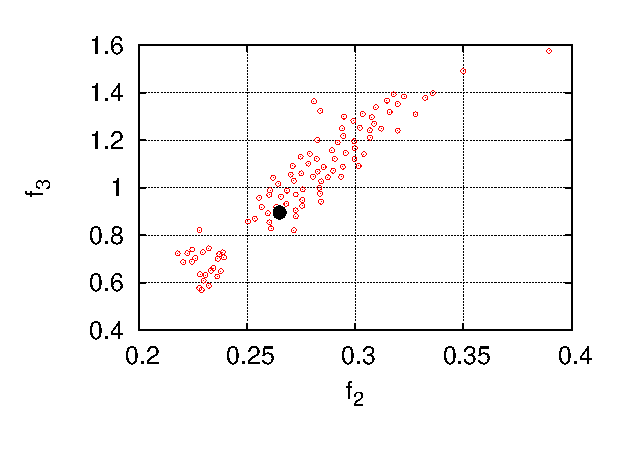
\includegraphics{./3obj6/final_pareto2d2.eps}}
\end{minipage}
\begin{minipage}[b]{0.5\linewidth}
 \centering
 \resizebox*{8.0cm}{!}{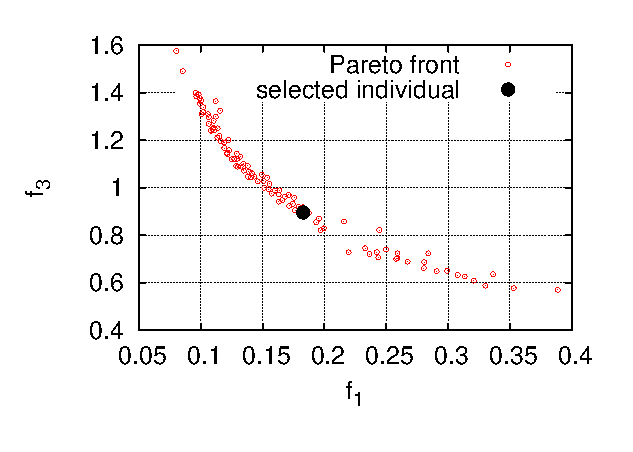
\includegraphics{./3obj6/final_pareto2d3.eps}}
\end{minipage}
\begin{minipage}[b]{0.5\linewidth}
 \centering
 \resizebox*{8.0cm}{!}{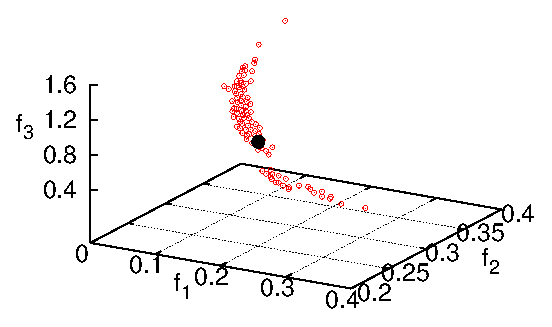
\includegraphics{./3obj6/final_pareto.eps}}
\end{minipage}
\begin{minipage}[b]{0.5\linewidth}
 \centering
 \resizebox*{8.0cm}{!}{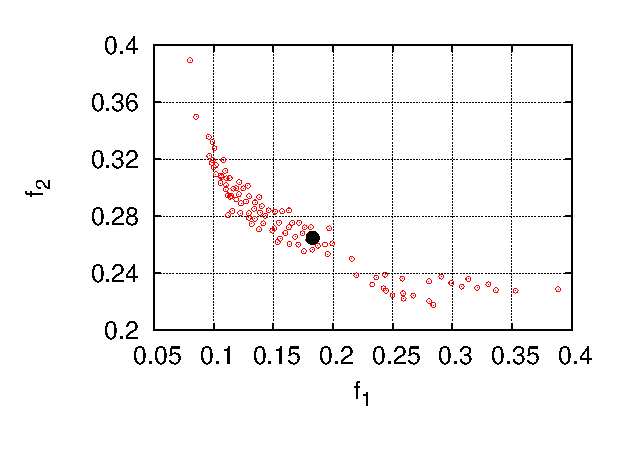
\includegraphics{./3obj6/final_pareto2d1.eps}}
\end{minipage}
\caption{Experimental validation of the design of a Hydromatrix$\circledR$: The 3D front of non-dominated solutions computed at the cost of 2000 evaluations and the design selected to undergo construction and  experimental validation. The 3D plot and its projections onto the ($(f_2,f_3)$, $(f_1,f_3)$ and $(f_1,f_2)$ planes) are shown.}
\label{exp.pareto}
\end{figure}

For the experimental validation, a single design from the computed front of non-dominated solutions was selected, manufactured and measured in test rig L2b of Andritz Hydro GmbH in Linz, Austria (fig.\ \ref{exp.lab}). The selected design is compared, efficiency-wise, with a reference Hydromatrix$\circledR$ turbine designed to operate at a ``similar'' operating region.    

Before proceeding to the experimental validation, an analysis of the numerical simulations performed for the selected design follows. In fig.\ \ref{exp.BE} (left), the high loading quality of the selected design is demonstrated through the $C_p$ chordwise distribution (eq.\ \ref{Cpdef}) along the hub, mid-span and shroud. In fig.\ \ref{exp.BE} (right), the excellent agreement of the outlet velocity profiles ($C_m$ and $C_u$) with the desired ones is presented. Furthermore, in fig.\ \ref{exp.PL.FL}, the $C_p$ distributions demonstrate the loading quality of the selected design when it operates at the FL and PL operating points.    

%\begin{figure}[h!]
%\begin{minipage}[b]{1\linewidth}
% \centering
% \resizebox*{15.0cm}{!}{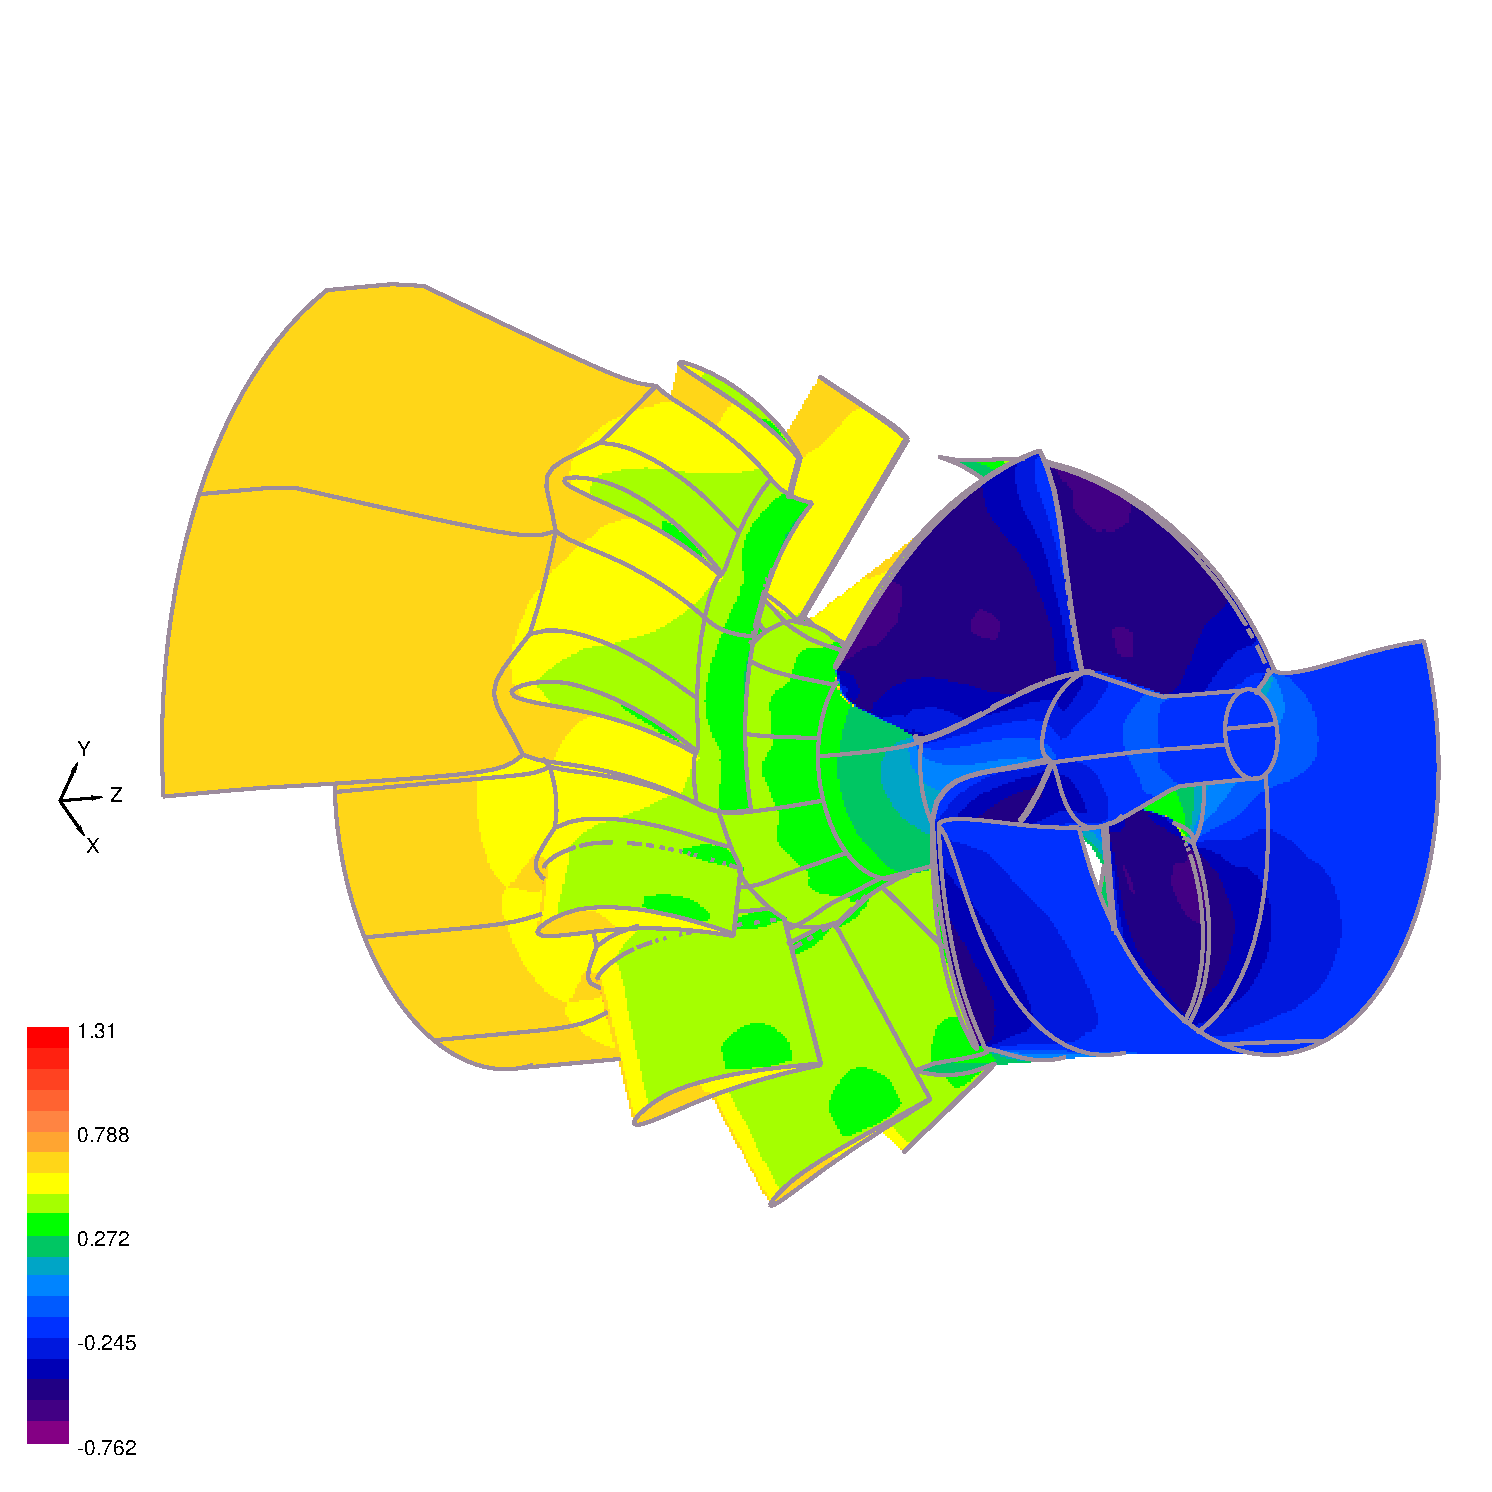
\includegraphics{./3obj6/OP1/AllPress.eps}}
%\end{minipage}
%\caption{Experimental validation of the design of a Hydromatrix$\circledR$: $\sigma$ contour for design A at BE operating point.}
%\label{exp.All_press.BE}
%\end{figure}


\begin{figure}[h!]
\begin{minipage}[b]{0.5\linewidth}
 \centering
 \resizebox*{7.5cm}{!}{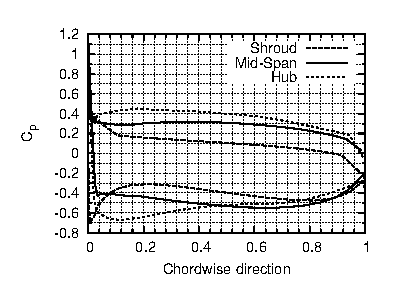
\includegraphics{./3obj6/OP1/LOAD.eps}}
\end{minipage}
\begin{minipage}[b]{0.5\linewidth}
 \centering
 \resizebox*{7.5cm}{!}{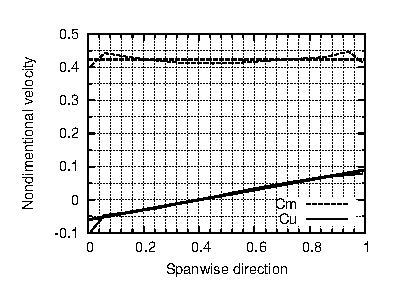
\includegraphics{./3obj6/OP1/OUTLET.eps}}
\end{minipage}

\caption{Experimental validation of the design of a Hydromatrix$\circledR$: Left: Computed $C_p$ profiles at hub, mid-span and shroud for the selected design operating at the BE point. Right: Computed $C_m$ and $C_u$ outlet velocity profiles for the selected design, at the BE point.}
\label{exp.BE}
\end{figure}
 
 

\begin{figure}[h!]
\begin{minipage}[b]{0.5\linewidth}
 \centering
 \resizebox*{7.5cm}{!}{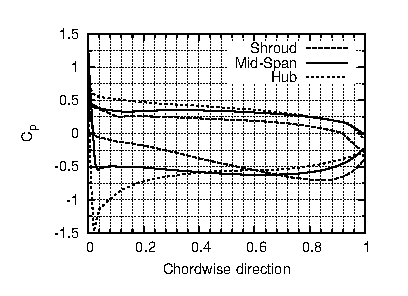
\includegraphics{./3obj6/OP2/LOAD.eps}}
\end{minipage}
\begin{minipage}[b]{0.5\linewidth}
 \centering
 \resizebox*{7.5cm}{!}{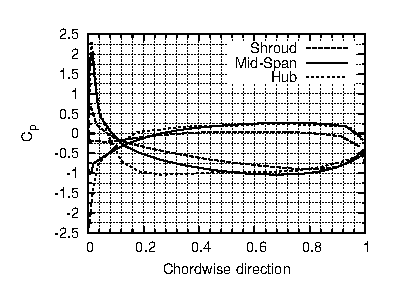
\includegraphics{./3obj6/OP3/LOAD.eps}}
\end{minipage}

\caption{Experimental validation of the design of a Hydromatrix$\circledR$: Computed $C_p$ profiles at hub, mid-span and shroud for the selected design operating at the FL point.  Right: Computed $C_p$ profiles at hub, mid-span and shroud for the same design, at the PL point}
\label{exp.PL.FL}
\end{figure}

\FloatBarrier
\section{Experimental Validation}  
The experimental validation of the  quality of the selected Hydromatrix$\circledR$ design was performed at the test rig L2b (fig.\ \ref{exp.lab}) which is specialized for Bulb, Straflo and Hydromatrix$\circledR$ turbines. In L2b, three pumps are used to simulate the desirable river flow (Q, H).  The model turbine is installed between  head- and tail-water tanks.

The model head is regulated by the pump speed and the tail
water elevation by the pressure in the downstream tank. The latter is connected to a vacuum vessel and compressed air. This allows varying the downstream tank pressure for the simulation of the necessary cavitation conditions, while keeping the model head constant. For the Hydromatrix$\circledR$ tests, a special inlet box to simulate the river flow is required.

\begin{figure}[h!]
\centering
\resizebox*{15.0cm}{!}
{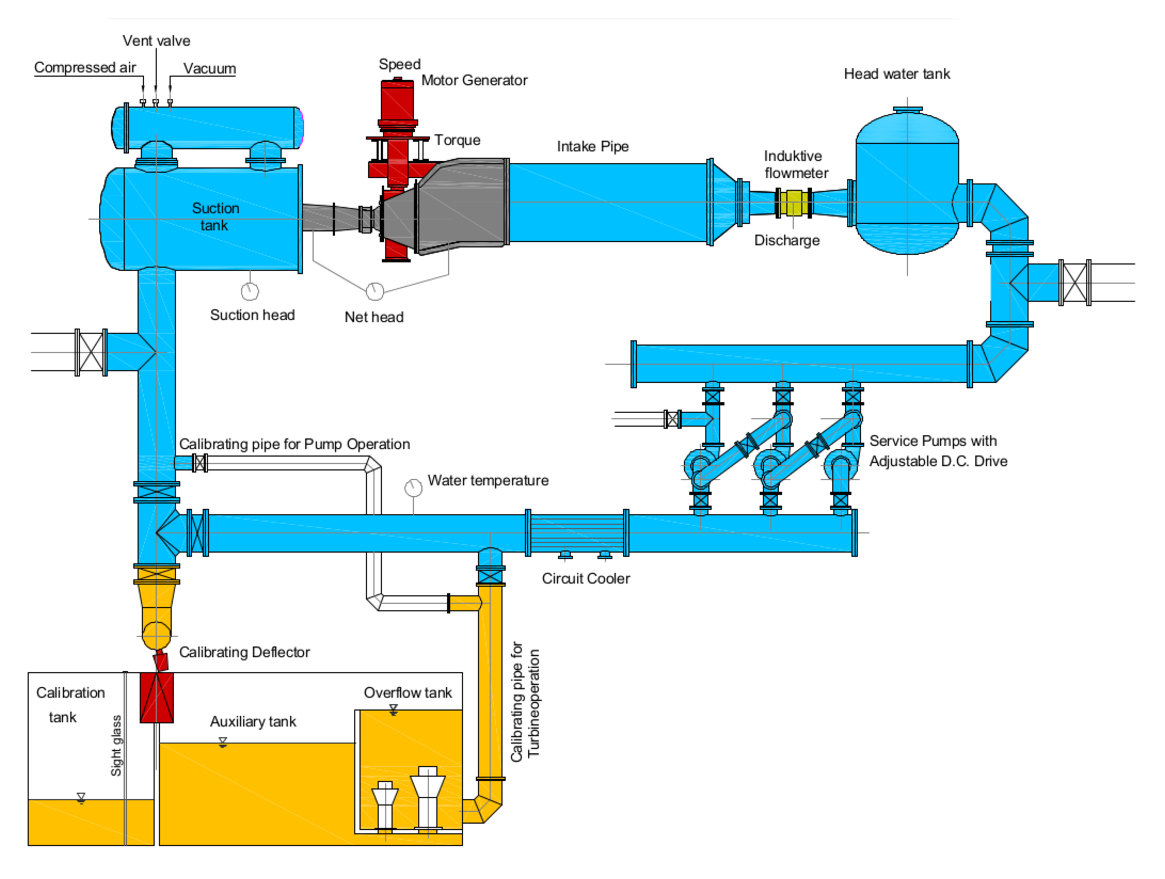
\includegraphics[width=1\textwidth]{lab.eps}}
\caption{Experimental validation of the design of a Hydromatrix$\circledR$: General layout of test rig L2b of Andritz-Hydro/Linz in the Hydromatrix$\circledR$ configuration.
L2b is operated as a closed loop and is able to perform a variety of tests in accordance with international standards ``IEC 60193" \cite{IEC}.}
\label{exp.lab}
\end{figure}

Regarding the torque measurement, a strain-gage equipped shaft, with its signal being transmitted via a wireless telemetry system to the data acquisition system is used. The model head (H) is computed from the static pressure difference between the head-water and tail-water tanks and the velocity difference between the measurement sections (distributor cone inlet and draft tube outlet). Volume flow rate Q is measured using an inductive discharge flowmeter; rotational speed is measured using an incremental encoder with a resolution of $1024$ impulses per revolution. All measuring instruments were calibrated either by primary normals or by using calibration devices which are calibrated with a primary normal. The runner blade geometry was checked with a 3D coordinate measurement machine by an external company.

\begin{figure}[h!]
\centering
\resizebox*{13.0cm}{!}
{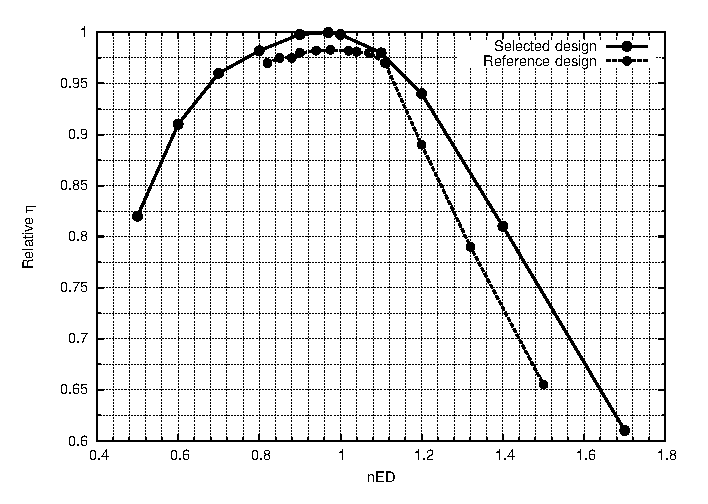
\includegraphics[width=1\textwidth]{./3obj6/Eff.eps}}
\caption{Experimental validation of the design of a Hydromatrix$\circledR$: Relative efficiency ($\frac{\eta}{max(\eta)}$) charts for the reference and the selected design. The selected design, optimized using the proposed  methods, outperforms the reference one throughout the operating spectrum.}
\label{exp.eff}
\end{figure}


Efficiency ($\eta$) measurements were performed at the minimum model Reynolds number of $4 × 10^6$ and minimum specific hydraulic energy of $30J/kg$, as indicated in IEC 60193 \cite{IEC}.
In order to acquire the efficiency curve, head and speed were changing so as to make the speed factor $N_{ED}$ vary too.  The measured efficiency of the selected design is shown, in comparison with a reference design, in fig.\ \ref{exp.eff}.    

The experimental validation showed that the methods proposed in this thesis deliver high quality designs, acceptable by industrial standards. Furthermore, the overall design time reduced from approximately $120-140$ days to only $50$. This reduction in time and, therefore, resources, combined with the ability to treat turbine parts, such the draft tube, as standardised components (merely requiring  their coupling properties) resulted in the reduction of the overall cost per unit to, approximately,  one third.

This cost reduction makes the use of this type of turbines, in power plants with even lower H (below 5m, as low as 2m)  and relatively small (smaller than $60m^3/s$) discharges, viable. The economic impact of this improvement can be very important as the current estimations for the potential of sites in the range of 2 to 5m is approximately $6000$ GWh
per year in Europe alone\footnote{This figure was given by ``European Commission, Joint Research Centre, Institute for Energy, Energy Systems Evaluation Unit,  Petten, 13 of June 2007'' in  ``Report on the Workshop on Hydropower and Ocean Energy – Part II: Hydropower''.}, a market worth potentially more than a billion Euro per year. 

  

 





 




% ---------------------------------------------------------------------------
%: ----------------------- end of thesis sub-document ------------------------
% ---------------------------------------------------------------------------



 






